\subsubsection{I2C Klassen}	\label{sec:I2C_design}

Der er designet en \IIC protokol (side \pageref{P-sec:I2C_protokol} i dokumentationen), som dækker over samtlige kommandoer der kan sendes.
Protokollen er designet med rige udvidelsesmuligheder, således er kommandoerne mulige at ændre, hvis der stødes på problemer med nogle af dem, eller hvis der er behov for at udvide funktionaliteten.

\begin{figure}[h]
\centering 
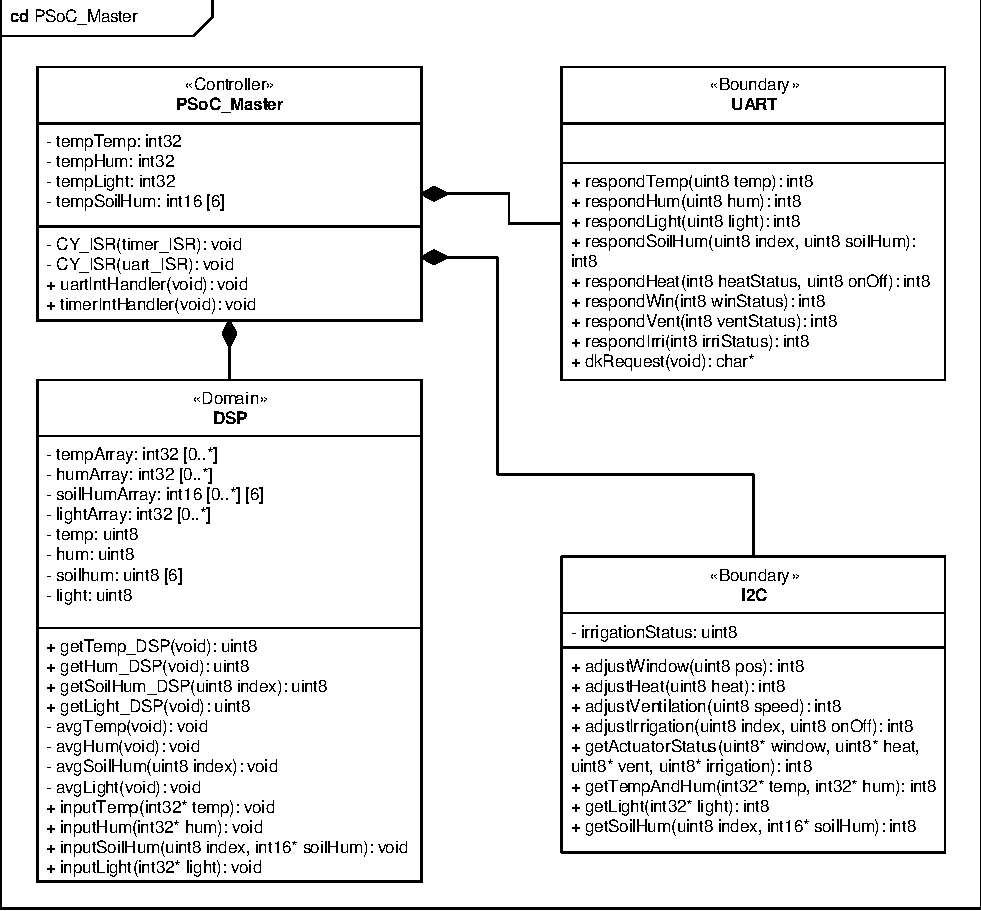
\includegraphics[width=\textwidth * 2/5, trim=269 27 17 267, clip=true] {../fig/cd_PSoC_master.pdf}
\caption{I2C klassen.}
\label{fig:i2C_klasse}
\end{figure}

Klassen \IIC står for indhentning og afsending af data fra/til hhv. sensorer og aktuatorer. Som det kan ses i klassediagrammet på Figur \ref{fig:i2C_klasse} er der designet metoder, hvis navne svarer til kommandoer. Formålet med klassen er, at varetage kommunikation på \IIC bussen. Eksempelvis varetager \texttt{adjustHeat()} metoden den kommunikation til Aktuator-slaven, når der skal slukkes eller tændes for varmelegemet. Metodens returværdi afspejler om kommunikationen gik godt, og at slaven har forstået beskeden.